\section{}

Wir nutzen die bisherige \texttt{newton}-Methode, kombiniert mit einer Approximation für Ableitungen:

\lstinputlisting[style=pythoncode, firstline = 1, lastline = 28]{chapter_04/exercise_04_14.py}

Wir plotten nun zunächst die gegeben Funktion
\[
  f(x) = e^x + 2x
\]
mit dem folgenden Code:

\lstinputlisting[style=pythoncode, firstline = 31, lastline = 43]{chapter_04/exercise_04_14.py}

Wir erhalten den folgenden Graphen:

\begin{center}
  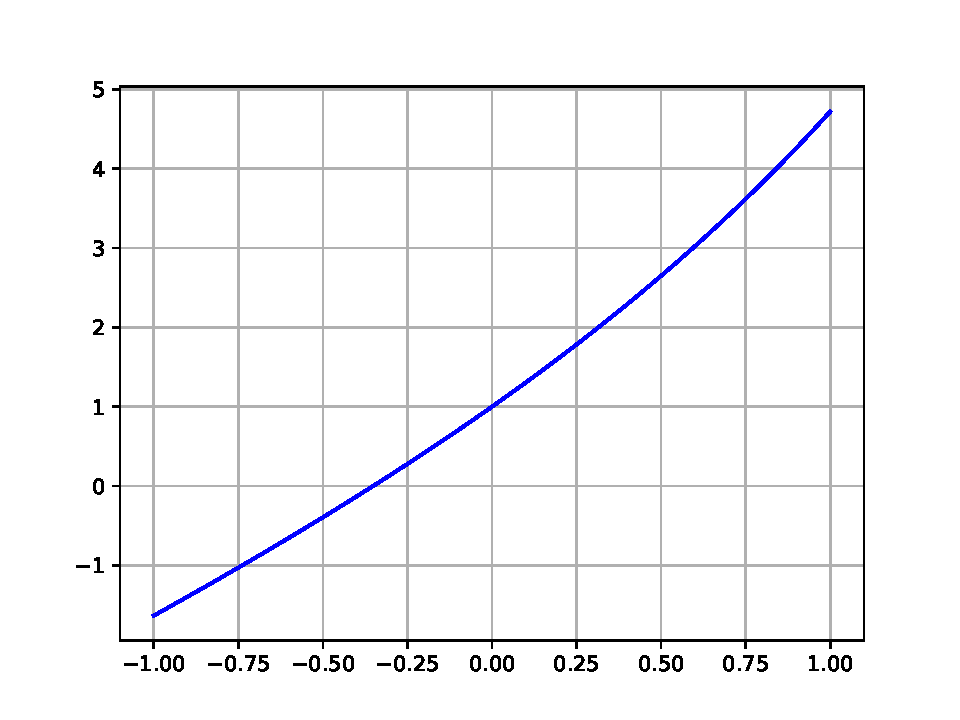
\includegraphics[width = 0.5\textwidth]{chapter_04/exercise_04_14_figure.pdf}
\end{center}

Wir wählen nun den Startwert $x_0 = 1$, und berechnen die Nullstelle von $f$ sowohl mit der bisherigen \texttt{newton}-Funktion, als auch mit der neuen \texttt{newton\_ext}-Funktion:

\lstinputlisting[style=pythoncode, firstline = 45, lastline = 48]{chapter_04/exercise_04_14.py}

Wir erhalten in der Konsole den folgenden Output:

\begin{consoleoutput}
With the exact derivative we get a root at      -0.35173371124919584.
With an approximate derivative we get a root at -0.35173371124919584.
\end{consoleoutput}
